\subsection{Functional Requirements}
The functionality for the various users.
\subsubsection {Requirements List}
\begin{enumerate}[label=\textbf{R\arabic*}]
\item PowerEnjoy shall provide Users with the ability to access all the System functionalities reserved to them.
\item PowerEnjoy shall support Users in locating Available Cars within a range of 5 Km from a specific position.
\item PowerEnjoy shall support Users in locating Parking Areas and their free parking slots.
\item PowerEnjoy shall support Users in locating Charging Areas and their free parking slots and free charging sockets.
\item PowerEnjoy shall support Users in reserve Available Cars.
\item PowerEnjoy shall apply a fixed Surcharge of 1 EUR if he/she has reserved a Car and not unlocked it within a time range of 60 minutes.
\item PowerEnjoy shall support a User in unlock a Car he/she has previously reserved when he/she is in a range of 15 meters from the same Car.
\item PowerEnjoy shall charge the User of a fixed fee per minutes, communicating to him/her the Fee he will get charged at the end of the ride basing only on the driving time and the fee per minutes.
\item PowerEnjoy shall be able to know if a User has took in the Car he/she is driving at least two other passengers for at least 3 minutes. If so, PowerEnjoy should apply a percentage Discount of 10\% on the final Fee of the last ride.
\item PowerEnjoy shall allow the User to end the ride in a Parking or Charging Area. 
\item PowerEnjoy shall allow any User who has ended a ride to plug the Car he/she has driven to a Socket in a time rage of 2 minutes since he/she has ended the ride, in order to get a percentage Discount of 30\% on the final Fee of the last ride.
\item PowerEnjoy shall apply a percentage Discount of 20\% on the final Fee of the last ride if the User will end the ride leaving the Car with more than 50\% battery charge status.
\item PowerEnjoy shall apply a percentage Surcharge of 30\% on the final Fee of the last ride if a User leaves the Car at more than 3 km from the nearest Charging Area or with a battery charge status less than 20\%.
\item PowerEnjoy shall provide a User the ability to use the "Money Saving Option", telling him/her the position of a Charging Area where he/she has to park the Car he/she is driving in order to get a Discount on the total Fee. The Charging Area is determined by the System to ensure a uniform distribution of Cars in the city of that address and depends both on the destination of the User and on the availability of Sockets at the selected Charging Area.
\item PowerEnjoy shall interface with an external Mailing System to send emails to Users.
\item PowerEnjoy shall interface with an external Banking System to charge Fee to Users.
\item PowerEnjoy shall interface with an external GPS System to know the positions of Users and Areas.
\item PowerEnjoy shall interface with an external Mapping System to know the positions of Users and Areas.
\item PowerEnjoy shall interface with the existing Car to get their GPS position, damages, connection to an electrical socket, the number of seats occupied. 
\end{enumerate}

\subsubsection{Use cases specification}
% Counter to use for UseCaseId
\newcounter{UseCaseIdCounter}

% It starts from 0 by default, so I've incremented it.
\stepcounter{UseCaseIdCounter}

\begin{longtable}{|p{0.2\linewidth} p{0.8\linewidth}|}
	% Some table settings
	\captionsetup{labelformat=empty} % To not show Table 1, Table 2 under the table
	\caption{\textbf{Register Account}} % Table caption
	\label{UC_Register}%If later on you want to refer to this label, you can this label. 
	\\ \hline % end of row + new horizontal line
	
	% The table itself
	\textbf{ID} & UC\theUseCaseIdCounter \\ \hline
	\textbf{Description} & The \emph{Visitor} wants to create an \emph{Account} for the \emph{Car-Sharing} Service. \\ \hline
	\textbf{Actors} & \emph{Visitor}.\\ \hline
	\textbf{Pre-Conditions} & The \emph{Visitor} connects to the \emph{Company's Car-Sharing}WebSite/Application. \\ \hline
	\textbf{Flow of events} & 
		\begin{enumerate}
			\item The \emph{Visitor} selects the function \textit{\textquotedblleft{Sign Up}\textquotedblright}.
			\item The \emph{System} returns a form to enter all the required data: Name, Surname, Birth date, ID Card Number, Driving License number and Credit Card number. It also asks for an email address and a password which will be used for the future logins.
			\item The \emph{Visitor} fills the form with all the required information.
			\item The \emph{System} stores the request together with all the data provided with it, generates a random activation URL and asks the \emph{Mail System} to forward his/her URL to the email address of the \emph{Visitor}.
		\end{enumerate}	 \\ \hline
	\textbf{Post Conditions} & The \emph{Mail System} sends the activation URL to the \emph{Visitor}'s email provided in the registration form. \\ \hline
	\textbf{Exceptions} & 
		\begin{itemize}
		\item The \emph{System} recognizes invalid or missing data in the form compiled by the emph{Visitor}and informs him/her of the error. The flow of events restarts from point 1.
		\item The Visitor inserts in the form a Social Security Number, or ID Card Number, or Driving License number, or Email Address, which is already present in the System. The System shows an error message saying that some of those credentials were already been inserted into the System for another account. The flow of events restarts from point 1.
		\end{itemize} \\ \hline
\end{longtable}


\stepcounter{UseCaseIdCounter}
\begin{longtable}{|p{0.2\linewidth} p{0.8\linewidth}|}
	% Some table settings
	\captionsetup{labelformat=empty} % To not show Table 1, Table 2 under the table
	\caption{\textbf{Activate Account}} % Table caption
	\label{UC_Activate}	\\ \hline
	
	% The table itself
	\textbf{ID} & UC\theUseCaseIdCounter \\ \hline
	\textbf{Description} & The \emph{Visitor} wants to activate his/her \emph{Account}. \\ \hline
	\textbf{Actors} & \emph{Visitor}.\\ \hline
	\textbf{Pre-Conditions} & The \emph{Visitor} has received the activation URL on his/her mail box. \\ \hline
	\textbf{Flow of ev-ents} & 
	\begin{enumerate}
		\item The \emph{Visitor} opens the received activation URL.
		\item The \emph{System} acknowledges that the Visitor has arrived in his/her activation Web Page and activates his/her account.
	\end{enumerate}	 \\ \hline
	\textbf{Post Conditions} & The \emph{Visitor} is now become an \emph{User} which can access the \emph{System} using the credentials (Email, password) he provided during the registration phase. \\ \hline
	\textbf{Exceptions} & 
	\begin{itemize}
		\item The Activation URL expires after 10 days it has been generated. The Visitor?s data are cancelled from the System and the Visitor will have to perform the Registration (UC1) again.
	\end{itemize} \\ \hline
\end{longtable}

\stepcounter{UseCaseIdCounter}

\begin{longtable}{|p{0.2\linewidth} p{0.8\linewidth}|}
	% Some table settings
	\captionsetup{labelformat=empty} % To not show Table 1, Table 2 under the table
	\caption{\textbf{Log In}} % Table caption
	\label{UC_Login}%If later on you want to refer to this label, you can use this label. 
	\\ \hline % end of row + new horizontal line
	
	% The table itself
	\textbf{ID} & UC\theUseCaseIdCounter \\ \hline
	\textbf{Description} & The \emph{Visitor} wants to log in the \emph{System}. \\ \hline
	\textbf{Actors} & \emph{Visitor}.\\ \hline
	\textbf{Pre-Conditions} & The \emph{Visitor} connects to the Company's \emph{Car-Sharing WebSite/Application} \\ \hline
	\textbf{Flow of events} & 
	\begin{enumerate}
		\item The \emph{Visitor} selects the function \textit{\textquotedblleft{Login}\textquotedblright} .
		\item The \emph{System} shows the \emph{Visitor} a login form, asking him to insert the email and password provided in the registration form.
		\item The \emph{Visitor} inserts the pair (Email,Password) used during the registration phase and selects the function \textit{\textquotedblleft{Log me in}\textquotedblright}
	\end{enumerate}	 \\ \hline
	\textbf{Post Conditions} & The \emph{System} verifies the existence of an account associated with that pair (Email,password) and logs the \emph{Visitor} in. The \emph{Visitor} has now become \emph{User}  \\ \hline
	\textbf{Exceptions} & 
	\begin{itemize}
		\item The Activation URL expires after 10 days it has been generated. The Visitor?s data are cancelled from the System and the Visitor will have to perform the Registration (UC1) again.
	\end{itemize} \\ \hline
\end{longtable}
\stepcounter{UseCaseIdCounter}

\begin{longtable}{|p{0.2\linewidth} p{0.8\linewidth}|}
	% Some table settings
	\captionsetup{labelformat=empty} % To not show Table 1, Table 2 under the table
	\caption{\textbf{Log Out}} % Table caption
	\label{UC_Logout}%If later on you want to refer to this label, you can use this label. 
	\\ \hline % end of row + new horizontal line
	
	% The table itself
	\textbf{ID} & UC\theUseCaseIdCounter \\ \hline
	\textbf{Description} & The User wants to log out from the System. \\ \hline
	\textbf{Actors} & \emph{User}.\\ \hline
	\textbf{Pre-Conditions} & The \emph{User} is logged in the \emph{System} \\ \hline
	\textbf{Flow of events} & 
	\begin{enumerate}
		\item The \emph{User} selects the function \textit{\textquotedblleft{Log out}\textquotedblright} .
		\item The \emph{System} performs the \emph{User}'s logout.
	\end{enumerate}	 \\ \hline
	\textbf{Post Conditions} & The \emph{System} shows the confirmation of the logout to the \emph{User}.
	
	The \emph{User} is now not able to use the \emph{System} functionalities dedicated to Users anymore (until he logs in again). \\ \hline
	\textbf{Exceptions} &  \\
%	\begin{itemize}
%	\end{itemize} \\ 
\hline
\end{longtable}
\stepcounter{UseCaseIdCounter}

\begin{longtable}{|p{0.2\linewidth} p{0.8\linewidth}|}
	% Some table settings
	\captionsetup{labelformat=empty} % To not show Table 1, Table 2 under the table
	\caption{\textbf{Locate Available Cars}} % Table caption
	\label{UC_LocateCars}%If later on you want to refer to this label, you can use this label. 
	\\ \hline % end of row + new horizontal line
	
	% The table itself
	\textbf{ID} & UC\theUseCaseIdCounter \\ \hline
	\textbf{Description} & The \emph{User} wants to locate the avialable \emph{Cars}. \\ \hline
	\textbf{Actors} & \emph{User}.\\ \hline
	\textbf{Pre-Conditions} & The \emph{User} is logged in the \emph{System} \\ \hline
	\textbf{Flow of events} & 
	\begin{enumerate}
		\item The \emph{User} selects the function \textit{\textquotedblleft{Locate Cars}\textquotedblright}.
		\item The \emph{System} shows a text box asking the \emph{User} to provide an address near which they would like to see the \emph{Cars} whose state is \textit{Available}.
		\item The \emph{User} inserts the desired address and selects the \textit{\textquotedblleft{Locate}\textquotedblright} function.
	\end{enumerate}	 \\ \hline
	\textbf{Post Conditions} & The \emph{System} shows the \emph{User} a map containing all the \emph{Cars} whose state is Available and which are within a 5KM range from the provided address. \\ \hline
	\textbf{Alternative Flow of Events} & The \emph{User} selects the function \textit{\textquotedblleft{Near Me}\textquotedblright} instead of inserting a specific address and sends their \emph{GPS Coordinates} to the \emph{System}. \\ \hline
	\textbf{Exceptions} & 
	\begin{itemize}
		\item The System does not find the inserted address and informs the User. The Flow of Events starts from point 1.
		\item There are no available Cars in the specified address/User?s Position. The System informs the User. The Flow of Events start from point 1.
	\end{itemize} \\ \hline
\end{longtable}
\stepcounter{UseCaseIdCounter}

\begin{longtable}{|p{0.2\linewidth} p{0.8\linewidth}|}
	% Some table settings
	\captionsetup{labelformat=empty} % To not show Table 1, Table 2 under the table
	\caption{\textbf{Reserve Available Car}} % Table caption
	\label{UC_ReserveCar}%If later on you want to refer to this label, you can use this label. 
	\\ \hline % end of row + new horizontal line
	
	% The table itself
	\textbf{ID} & UC\theUseCaseIdCounter \\ \hline
	\textbf{Description} & The \emph{User} wants to reserve a \emph{Car}. \\ \hline
	\textbf{Actors} & \emph{User}.\\ \hline
	\textbf{Pre-Conditions} & The \emph{User} is logged in the \emph{System}, the \emph{User} does not have another active reservation, the \emph{User} is not driving another \emph{Car}, and the System has found available \emph{Cars} when the \emph{User} activated the \textit{\textquotedblleft{Locate Available Cars}\textquotedblright} function. \\ \hline
	\textbf{Flow of events} & 
	\begin{enumerate}
		\item The \emph{User} chooses a specific \emph{Car} among those showed on the map.
		\item The \emph{User} selects the function \textit{\textquotedblleft{Reserve this Car}\textquotedblright}.
	\end{enumerate}	 \\ \hline
	\textbf{Post Conditions} & The \emph{System} stores the \emph{Reservation} of the \emph{Car}, changing its status to \emph{Reserved}.
The \emph{System} activates a countdown of 1 hour during which the \emph{User} will have the possibility to unlock the \emph{Reserved} \emph{Car}. \\ \hline
	\textbf{Exceptions} & \\ \hline
\end{longtable}
\stepcounter{UseCaseIdCounter}

\begin{longtable}{|p{0.2\linewidth} p{0.8\linewidth}|}
	% Some table settings
	\captionsetup{labelformat=empty} % To not show Table 1, Table 2 under the table
	\caption{\textbf{Unlock Car}} % Table caption
	\label{UC_UnlockCar}%If later on you want to refer to this label, you can use this label. 
	\\ \hline % end of row + new horizontal line
	
	% The table itself
	\textbf{ID} & UC\theUseCaseIdCounter \\ \hline
	\textbf{Description} & The \emph{User} wants the \emph{System} to open the doors of the \emph{Car} in order to enter it. \\ \hline
	\textbf{Actors} & \emph{User}.\\ \hline
	\textbf{Pre-Conditions} & The \emph{User} is logged in the \emph{System} and has reserved a \emph{Car}. \\ \hline
	\textbf{Flow of events} & 
	\begin{enumerate}
		\item The \emph{User} activates the function\textit{\textquotedblleft{Unlock Car}\textquotedblright}.
		\item The \emph{User} sends their GPS coordinates to the \emph{System}.
		\item The \emph{System} checks that the GPS coordinates of the \emph{User} are within a 15 metres range from those of the \emph{Car} itself.
	\end{enumerate}	 \\ \hline
	\textbf{Post Conditions} & The \emph{System} has verified that the \emph{User} is nearby the car (within the specified distance range) and unlocks the \emph{Car}'s doors.
	 
The \emph{System} then changes the \emph{Car} status to \emph{In Use} and sets the \emph{Plugged} Flag to False.

The \emph{User} enters the \emph{Car}. \\ \hline
	\textbf{Exceptions} & If one hour has passed since the reservation has been made and the \emph{User} hasn't unlocked the Car, either because he wasn't within the 15 meters distance range or didn't activate this function, then:
	\begin{itemize}
	\item The reservation expires, so that the \emph{User} cannot unlock the \emph{Car} anymore (unless they reserve it again).
	\item The \emph{System} changes the \emph{Car}'s status to \emph{Available}.
	\item The \emph{System} communicates to the \emph{Banking System} the \emph{Fee} to charge the \emph{User} (this sum amounts to 1 EUR).
	\item The \emph{System} allows the \emph{User} to perform another reservation.
	\end{itemize} \\ \hline
\end{longtable}
\stepcounter{UseCaseIdCounter}

\begin{longtable}{|p{0.2\linewidth} p{0.8\linewidth}|}
	% Some table settings
	\captionsetup{labelformat=empty} % To not show Table 1, Table 2 under the table
	\caption{\textbf{Drive Car}} % Table caption
	\label{UC_DriveCar}%If later on you want to refer to this label, you can use this label. 
	\\ \hline % end of row + new horizontal line
	
	% The table itself
	\textbf{ID} & UC\theUseCaseIdCounter \\ \hline
	\textbf{Description} & The \emph{User} starts driving the \emph{Reserved} \emph{Car}. \\ \hline
	\textbf{Actors} & \emph{User}.\\ \hline
	\textbf{Pre-Conditions} & The \emph{User} has unlocked the doors of the \emph{Car} and entered it. \\ \hline
	\textbf{Flow of events} & 
	\begin{enumerate}
		\item The \emph{User} starts the engine of the \emph{Car}.
		\item The \emph{System} starts the Ride Timer which indicates the time usage of the \emph{Car}.
		\item {[}Extension Point UC 9{]}
		\item {[}Extension Point UC 12{]}
		\item The \emph{System} calculates the current \emph{Fee} charged to the \emph{User} (calculated as a given amount of money per minute on the Ride Timer) while showing it on the on-board screen.
	\end{enumerate}	 \\ \hline
	\textbf{Post Conditions} & The \emph{User} drives the \emph{Car} \\ \hline
	\textbf{Exceptions} & \\ \hline
\end{longtable}
\stepcounter{UseCaseIdCounter}

\begin{longtable}{|p{0.2\linewidth} p{0.8\linewidth}|}
	% Some table settings
	\captionsetup{labelformat=empty} % To not show Table 1, Table 2 under the table
	\caption{\textbf{Drive With Passengers $<<$extends UC 8$>>$}} % Table caption
	\label{UC_DriveWithPassengers}%If later on you want to refer to this label, you can use this label. 
	\\ \hline % end of row + new horizontal line
	
	% The table itself
	\textbf{ID} & UC\theUseCaseIdCounter \\ \hline
	\textbf{Description} & The \emph{User} picks up \emph{Passengers} to share the ride with. \\ \hline
	\textbf{Actors} & \emph{User}.\\ \hline
	\textbf{Pre-Conditions} & The \emph{User} is driving their \emph{Reserved} \emph{Car}. \\ \hline
	\textbf{Flow of events} & 
	\begin{enumerate}
		\item The \emph{User} picks up the \emph{Passengers}.
		\item The \emph{Car} detects the presence and number of the \emph{Passengers}.
	\end{enumerate}	 \\ \hline
	\textbf{Post Conditions} & The \emph{User} is sharing the ride with their \emph{Passengers}.
	
	The \emph{System} stores the number of \emph{Passengers} who were picked up and whether they stayed in the \emph{Car} for at least 3 minutes.\\ \hline
	\textbf{Exceptions} & \\ \hline
\end{longtable}
\stepcounter{UseCaseIdCounter}

\begin{longtable}{|p{0.2\linewidth} p{0.8\linewidth}|}
	% Some table settings
	\captionsetup{labelformat=empty} % To not show Table 1, Table 2 under the table
	\caption{\textbf{End Ride}} % Table caption
	\label{UC_EndRide}%If later on you want to refer to this label, you can use this label. 
	\\ \hline % end of row + new horizontal line
	
	% The table itself
	\textbf{ID} & UC\theUseCaseIdCounter \\ \hline
	\textbf{Description} & The \emph{User} ends the ride and the \emph{System} processes the \emph{Fee}. \\ \hline
	\textbf{Actors} & \emph{User}.\\ \hline
	\textbf{Pre-Conditions} & The \emph{User} parks the \emph{Car} in one of the \emph{Parking Areas}. \\ \hline
	\textbf{Flow of events} & 
	\begin{enumerate}
		\item The \emph{User} exits the \emph{Car}.
		\item The \emph{System} verifies that no one is in the \emph{Car}.
		\item The \emph{System} checks the \emph{Battery} status. 
		\item The \emph{System} checks, via the GPS coordinates, whether the \emph{User} has left the \emph{Car} within a 3KM distance range from the nearest \emph{Charging Area}.
		\item The \emph{System} checks if the \emph{User} drove with \emph{Passengers} (UC9).
		\item {[}Extension Point UC11{]}.
	\end{enumerate}	 \\ \hline
	\textbf{Post Conditions} & The \emph{System} locks the doors of the \emph{Car} and sets its status to \emph{Available}.
	
	The \emph{System} communicates to the \emph{Banking System} the final \emph{Fee} to charge the \emph{User}. \\ \hline
	\textbf{Alternative Flow of Events} & 
	\begin{itemize}
		\item The \emph{Battery} status is higher than 50\%, the \emph{User} didn't or did take at least 2 \emph{Passengers} with him for at least 3 minutes (UC9), didn't leave the \emph{Car} further than 3KM from the nearest \emph{Charging Area}, didn't plug the \emph{Car} (UC11), hence the System applies a 20\% \emph{Discount} on the \emph{Fee} of the last ride and communicates it to the \emph{Banking System} the \emph{Fee} which will be charged to the \emph{User}.
		\item The \emph{User} did plug the \emph{Car} (UC11), the \emph{Battery} status is higher than or equal to 20\%, they didn't or did take at least 2 \emph{Passengers} with him for at least 3 minutes (UC9), hence the System applies a 30\% \emph{Discount} on the \emph{Fee} of the last ride and communicates to the \emph{Banking System} the \emph{Fee} which will be charged to the \emph{User}.
		\item The \emph{User} did plug the \emph{Car} (UC11), the \emph{Battery} status is lower than 20\%, they didn't or did take at least 2 \emph{Passengers} with him for at least 3 minutes (UC9), hence the System doesn't apply any \emph{Discount} or \emph{Surcharge} on the \emph{Fee} of the last ride and communicates to the \emph{Banking System} the \emph{Fee} which will be charged to the \emph{User}.
		\item The \emph{User} didn't plug the \emph{Car} (UC11), the \emph{Battery} status is higher than 50\%, they either did or didn't take at least 2 \emph{Passengers} with him for at least 3 minutes (UC9), did leave the \emph{Car} further than 3KM from the nearest \emph{Charging Area}, hence the System applies a 10\% \emph{Surcharge} on the \emph{Fee} of the last ride and communicates to the \emph{Banking System} the \emph{Fee} which will be charged to the \emph{User}.
		% Even longtable can't handle tables this long
		\end{itemize} \\ &
		\begin{itemize}
		\item The \emph{Battery} status is between 20\% and 50\% (included), the \emph{User} did take at least 2 \emph{Passengers} with him for at least 3 minutes (UC9), didn't leave the \emph{Car} further than 3KM from the nearest \emph{Charging Area}, didn't plug the \emph{Car} (UC11), hence the System applies a 10\% \emph{Discount} on the \emph{Fee} of the last ride and communicates to the \emph{Banking System} the \emph{Fee} which will be charged to the \emph{User}.
		\item The \emph{Battery} status is lower than 20\%, the \emph{User} did take at least 2 \emph{Passengers} with him for at least 3 minutes (UC9), either did or didn't leave the \emph{Car} further than 3KM from the nearest \emph{Charging Area}, didn't plug the \emph{Car} (UC11), hence the System applies a 20\% \emph{Surcharge} on the \emph{Fee} of the last ride and communicates to the \emph{Banking System} the \emph{Fee} which will be charged to the \emph{User}.
		\item The \emph{Battery} status is between 20\% and 50\% (included), the \emph{User} did take at least 2 \emph{Passengers} with him for at least 3 minutes (UC9), did leave the \emph{Car} further than 3KM from the nearest \emph{Charging Area}, hence the System applies a 20\% \emph{Surcharge} on the \emph{Fee} of the last ride and communicates to the \emph{Banking System} the \emph{Fee} which will be charged to the \emph{User}.
		\item The \emph{Battery} status is lower than 20\%, the \emph{User} didn't take at least 2 \emph{Passengers} with him for at least 3 minutes (UC9), either did or didn't leave the \emph{Car} further than 3KM from the nearest \emph{Charging Area}, didn't plug the \emph{Car} (UC11), hence the System applies a 30\% \emph{Surcharge} on the \emph{Fee} of the last ride and communicates to the \emph{Banking System} the \emph{Fee} which will be charged to the \emph{User}.
		\end{itemize} \\ &
		\begin{itemize}
		\item The \emph{Battery} status is higher than 50\%, the \emph{User} either did or didn't take at least 2 \emph{Passengers} with him for at least 3 minutes (UC9), did leave the \emph{Car} further than 3KM from the nearest \emph{Charging Area}, didn't plug the \emph{Car} (UC11), hence the System applies a 10\% \emph{Surcharge} on the \emph{Fee} of the last ride and communicates to the \emph{Banking System} the \emph{Fee} which will be charged to the \emph{User}.	
		\item The \emph{Battery} status is between 20\% and 50\% (included), the \emph{User} didn't take at least 2 \emph{Passengers} with him for at least 3 minutes (UC9), did leave the \emph{Car} further than 3KM from the nearest \emph{Charging Area}, hence the System applies a 30\% \emph{Surcharge} on the \emph{Fee} of the last ride and communicates to the \emph{Banking System} the \emph{Fee} which will be charged to the \emph{User}.
	\end{itemize} \\ \hline
	\textbf{Exceptions} & If the \emph{Battery} status reaches 0\% of capacity or the \emph{Car} detects a major damage, the \emph{Car} stops and an assistance team is deployed. \\ \hline
\end{longtable}
\stepcounter{UseCaseIdCounter}

\begin{longtable}{|p{0.2\linewidth} p{0.8\linewidth}|}
	% Some table settings
	\captionsetup{labelformat=empty} % To not show Table 1, Table 2 under the table
	\caption{\textbf{Plug the Car $<<$extends UC 10$>>$}} % Table caption
	\label{UC_PlugCar}%If later on you want to refer to this label, you can use this label. 
	\\ \hline % end of row + new horizontal line
	
	% The table itself
	\textbf{ID} & UC\theUseCaseIdCounter \\ \hline
	\textbf{Description} & The \emph{User} plugs the \emph{Car} for recharging. \\ \hline
	\textbf{Actors} & \emph{User}.\\ \hline
	\textbf{Pre-Conditions} & The \emph{User} has parked the \emph{Car} in one of the \emph{Charging Areas} designated by the \emph{System}. \\ \hline
	\textbf{Flow of events} & 
	\begin{enumerate}
		\item The \emph{User} plugs the \emph{Car} into a \emph{Socket} of the \emph{Charging Area}. 
		\item The \emph{System} detects that the \emph{Car} has been plugged within 2 minutes since the \emph{User} got off the \emph{Car}.
	\end{enumerate}	 \\ \hline
	\textbf{Post Conditions} & The \emph{Battery} of the \emph{Car} is charging and the \emph{System} remembers the \emph{User}'s action for possible discounts.
	
The \emph{System} sets the \emph{Car}'s \emph{Plugged} flag to True.
	\\ \hline
	\textbf{Exceptions} & \\ \hline
\end{longtable}
\stepcounter{UseCaseIdCounter}

\begin{longtable}{|p{0.2\linewidth} p{0.8\linewidth}|}
	% Some table settings
	\captionsetup{labelformat=empty} % To not show Table 1, Table 2 under the table
	\caption{\textbf{Enable Money Saving Option $<<$extends UC 8$>>$}} % Table caption
	\label{UC_PlugCar}%If later on you want to refer to this label, you can use this label. 
	\\ \hline % end of row + new horizontal line
	
	% The table itself
	\textbf{ID} & UC\theUseCaseIdCounter \\ \hline
	\textbf{Description} & The \emph{User} asks the \emph{System} to suggest them a \emph{Charging Area} where to leave the \emph{Car}. \\ \hline
	\textbf{Actors} & \emph{User}.\\ \hline
	\textbf{Pre-Conditions} & The \emph{User} enables the \textit{\textquotedblleft{Money Saving}\textquotedblright} option. \\ \hline
	\textbf{Flow of events} & 
	\begin{enumerate}
		\item The \emph{System} asks the\emph{User} the destination address, providing them with a text box where to insert it.
		\item The \emph{User} provides the address to the \emph{System}.
	\end{enumerate}	 \\ \hline
	\textbf{Post Conditions} & The \emph{System} uses an algorithm which takes in consideration the distribution of the cars in the city, the final destination of the \emph{User} and the availability of power plugs in \emph{Charging Areas} to find the optimal \emph{Charging Area} for the \emph{User} to park their \emph{Car} in. The result of this algorithm will be sent to the \emph{User}, providing him the address of the \emph{Charging Area} where to leave the \emph{Car}. The \emph{User} will still have to plug the \emph{Car} in order to get a discount.
	\\ \hline
	\textbf{Exceptions} & If the \emph{Socket} of the \emph{Charging Area} has no more available plugs , the \emph{System} informs the \emph{User} and the Flow of Events starts from point 1.\\ \hline
\end{longtable}
\stepcounter{UseCaseIdCounter}

\subsubsection{Use Case Diagram}
\begin{figure}[h]
\centering
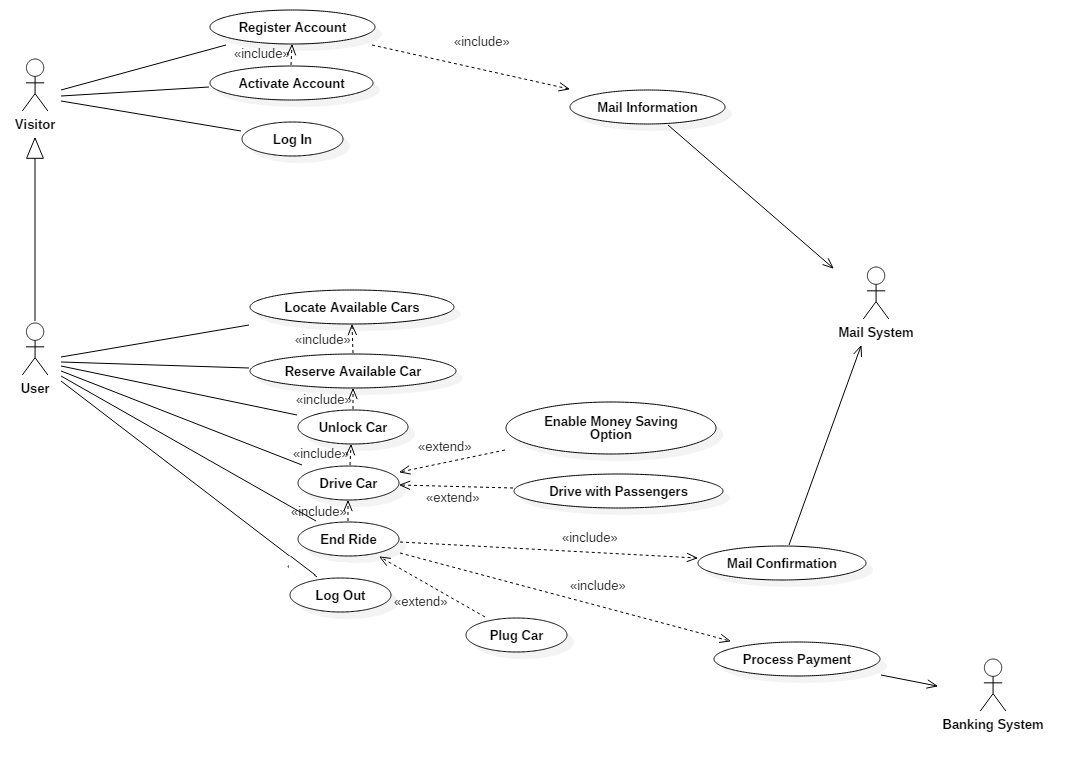
\includegraphics[width=\linewidth,keepaspectratio]{../Diagrams/UC/Use_Case.png}
\caption{Use Case}
\end{figure}
\FloatBarrier
\clearpage

\subsubsection{Activity Diagrams}
\begin{figure}[h]
\centering
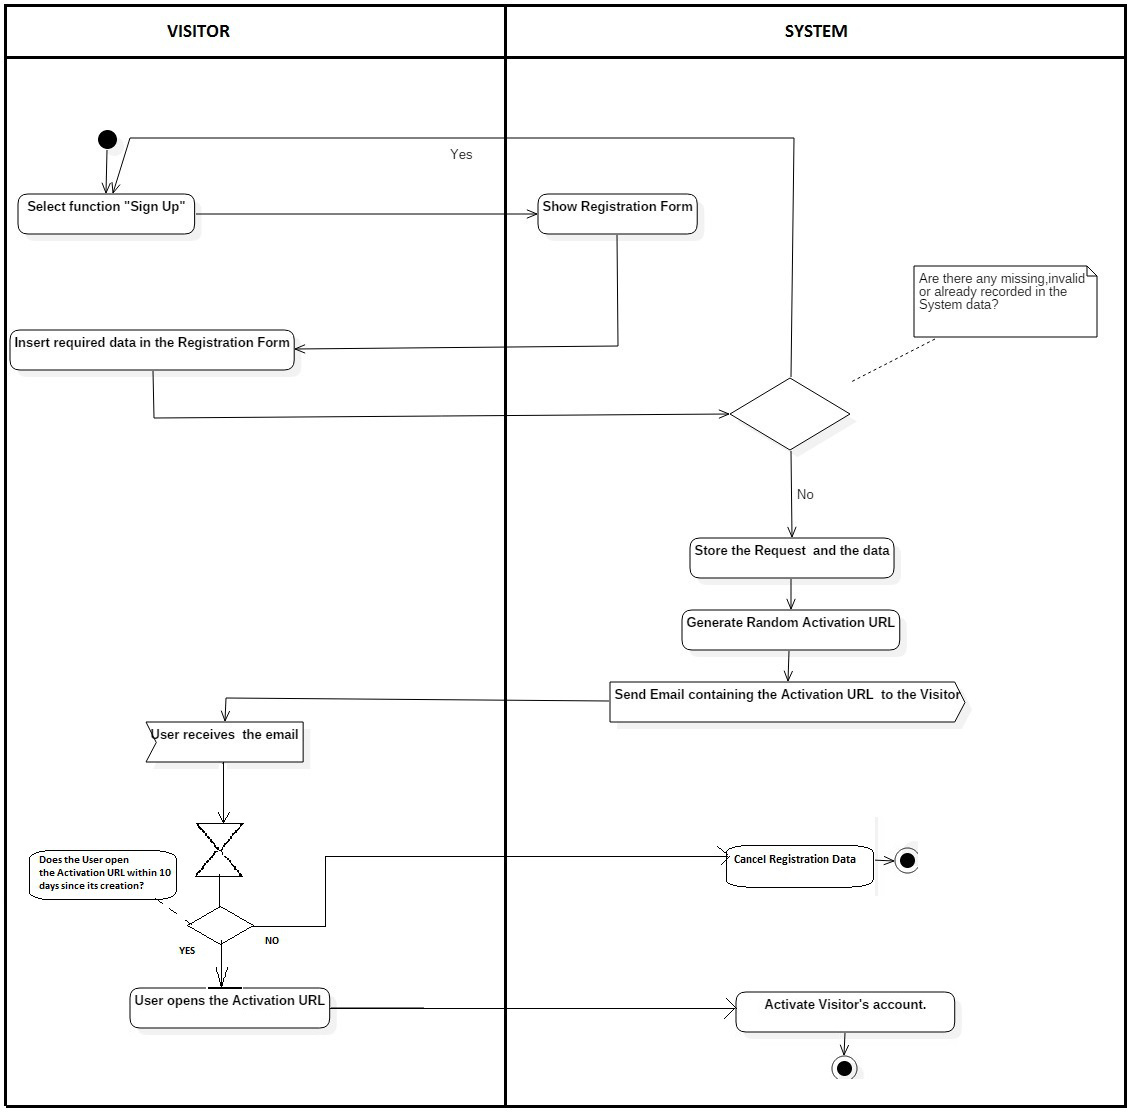
\includegraphics[width=\linewidth,keepaspectratio]{../Diagrams/AD/Registration.jpg}
\caption{Registration flowchart}
\end{figure}
\FloatBarrier
\begin{figure}[h]
\centering
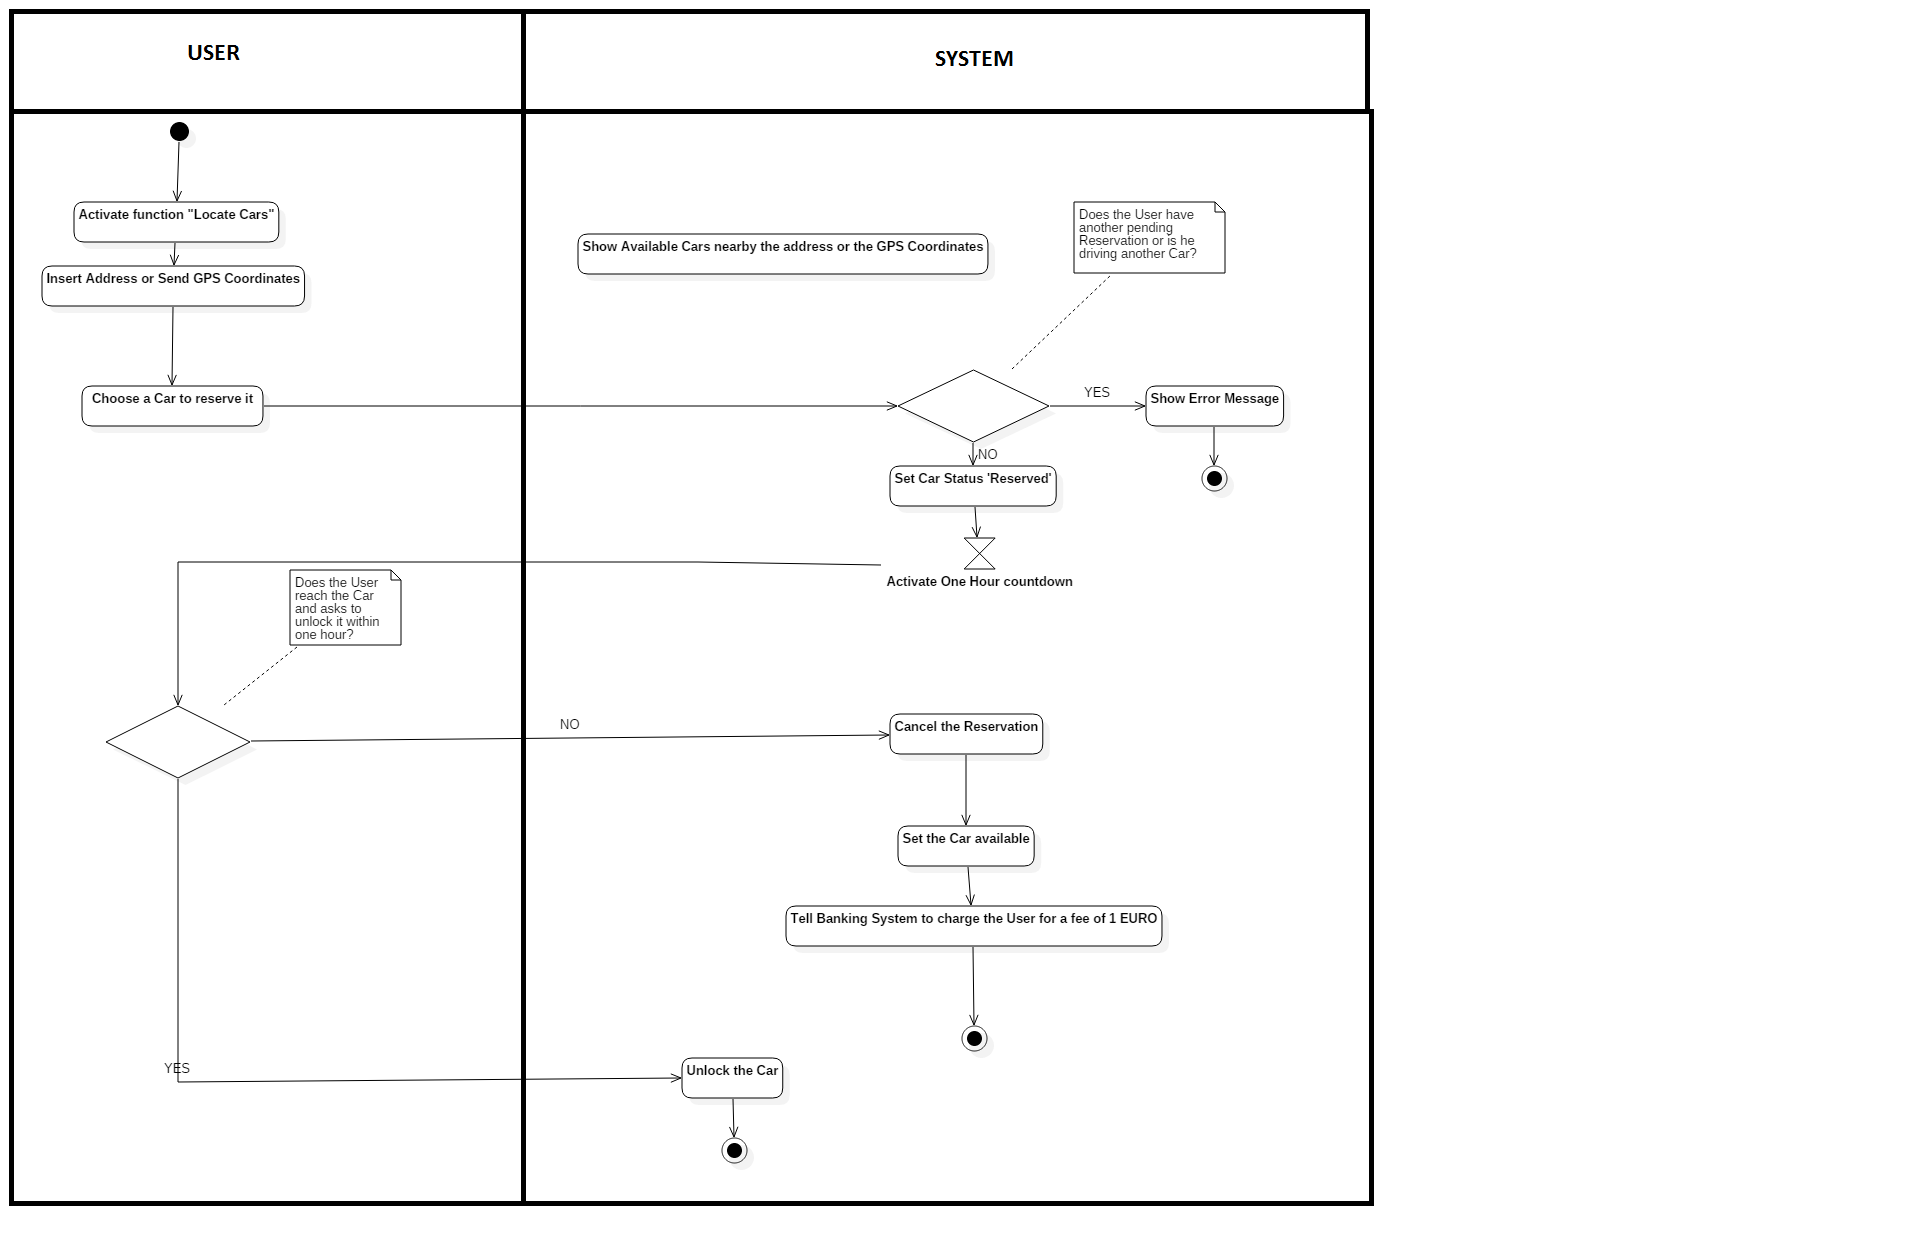
\includegraphics[width=\linewidth,keepaspectratio]{../Diagrams/AD/Locate_Reserve_Unlock.png}
\caption{Reservation flowchart}
\end{figure}
\FloatBarrier
\begin{figure}[h]
\centering
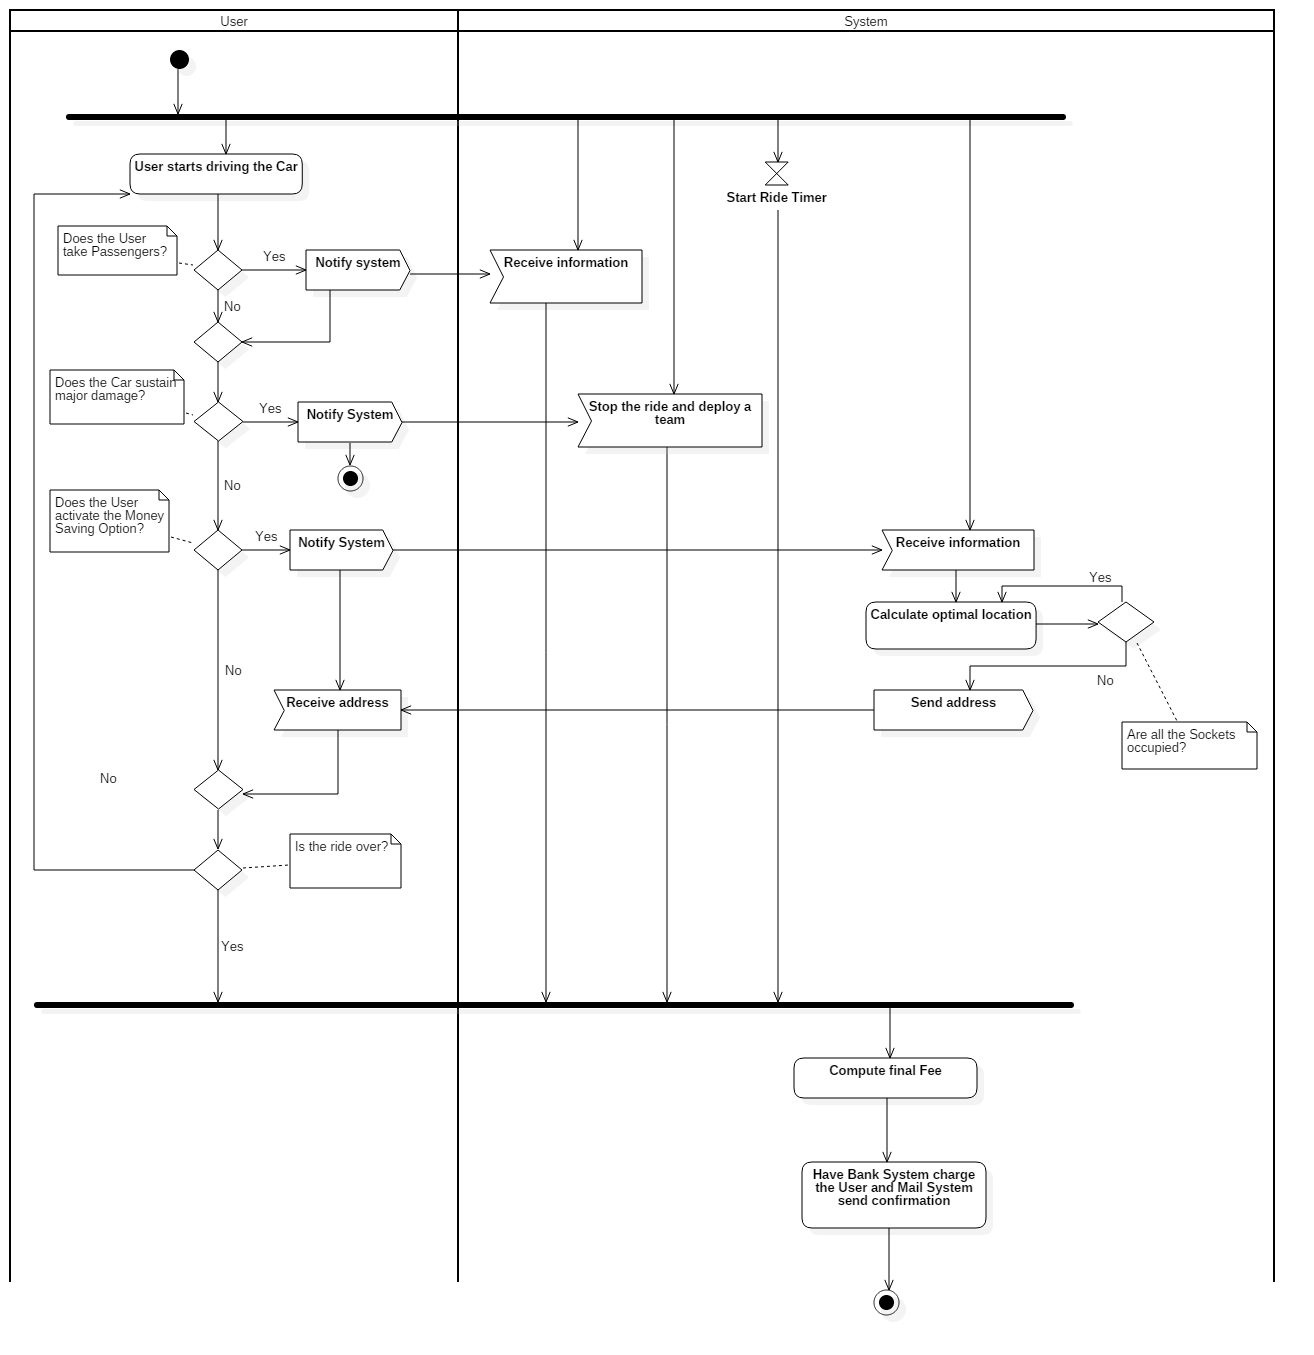
\includegraphics[width=\linewidth,keepaspectratio]{../Diagrams/AD/Ride.png}
\caption{Ride flowchart}
\end{figure}
\FloatBarrier

\subsubsection{Sequence Diagrams}
\begin{figure}[h]
\centering
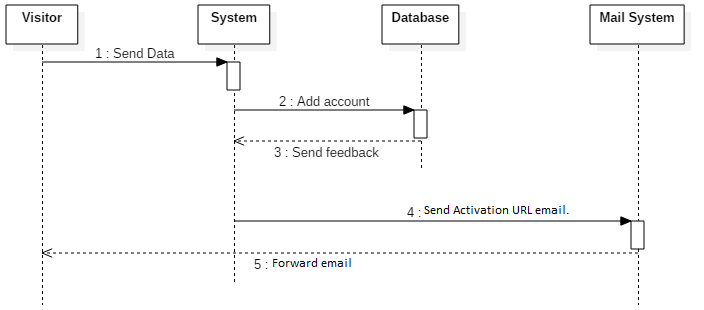
\includegraphics[width=\linewidth,keepaspectratio]{../Diagrams/SD/UC_1.png}
\caption{Use Case 1}
\end{figure}
\FloatBarrier
\begin{figure}[h]
\centering
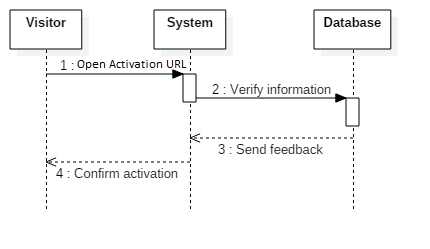
\includegraphics[width=\linewidth,keepaspectratio]{../Diagrams/SD/UC_2.png}
\caption{Use Case 2}
\end{figure}
\FloatBarrier
\begin{figure}[h]
\centering
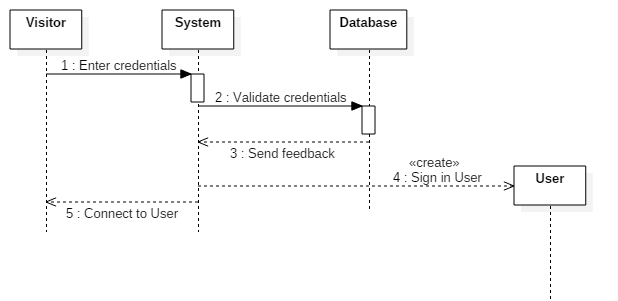
\includegraphics[width=\linewidth,keepaspectratio]{../Diagrams/SD/UC_3.png}
\caption{Use Case 3}
\end{figure}
\FloatBarrier
\begin{figure}[h]
\centering
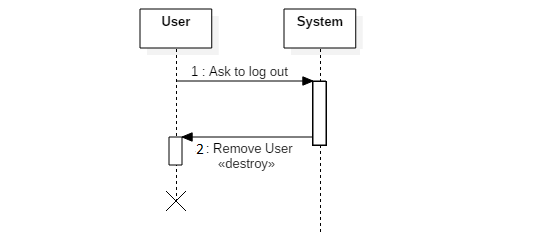
\includegraphics[width=\linewidth,keepaspectratio]{../Diagrams/SD/UC_4.png}
\caption{Use Case 4}
\end{figure}
\FloatBarrier
\begin{figure}[h]
\centering
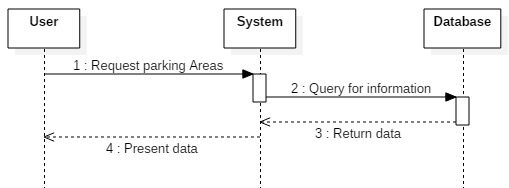
\includegraphics[width=\linewidth,keepaspectratio]{../Diagrams/SD/UC_5.png}
\caption{Use Case 5}
\end{figure}
\FloatBarrier
\begin{figure}[h]
\centering
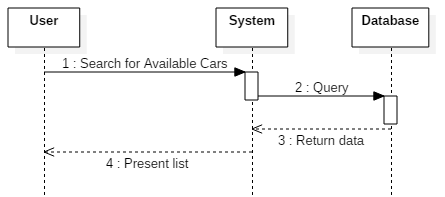
\includegraphics[width=\linewidth,keepaspectratio]{../Diagrams/SD/UC_6.png}
\caption{Use Case 6}
\end{figure}
\FloatBarrier
\begin{figure}[h]
\centering
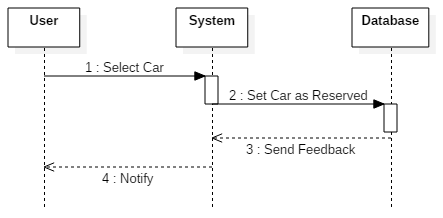
\includegraphics[width=\linewidth,keepaspectratio]{../Diagrams/SD/UC_7.png}
\caption{Use Case 7}
\end{figure}
\FloatBarrier
\begin{figure}[h]
\centering
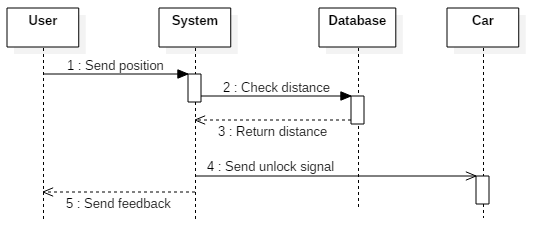
\includegraphics[width=\linewidth,keepaspectratio]{../Diagrams/SD/UC_8.png}
\caption{Use Case 8}
\end{figure}
\FloatBarrier
\begin{figure}[h]
\centering
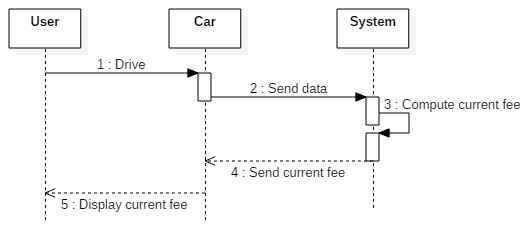
\includegraphics[width=\linewidth,keepaspectratio]{../Diagrams/SD/UC_9.png}
\caption{Use Case 9}
\end{figure}
\FloatBarrier
\begin{figure}[h]
\centering
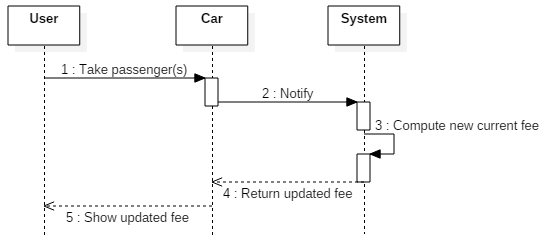
\includegraphics[width=\linewidth,keepaspectratio]{../Diagrams/SD/UC_10.png}
\caption{Use Case 10}
\end{figure}
\FloatBarrier
\begin{figure}[h]
\centering
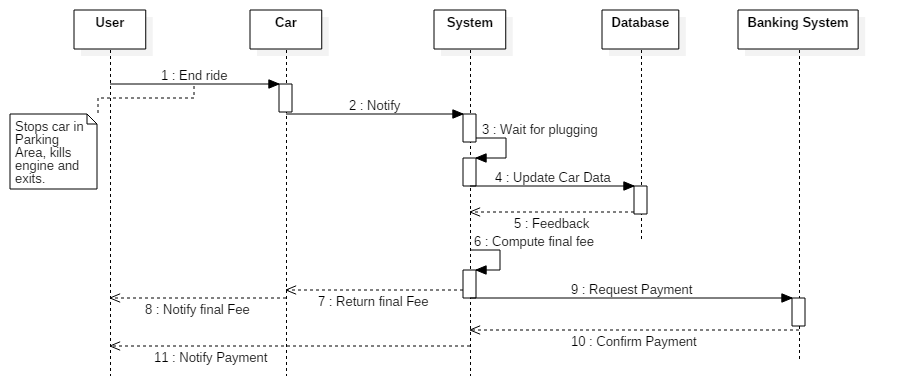
\includegraphics[width=\linewidth,keepaspectratio]{../Diagrams/SD/UC_11.png}
\caption{Use Case 11}
\end{figure}
\FloatBarrier
\begin{figure}[h]
\centering
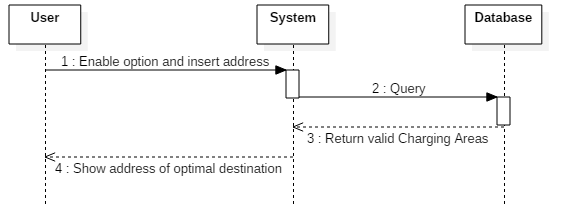
\includegraphics[width=\linewidth,keepaspectratio]{../Diagrams/SD/UC_12.png}
\caption{Use Case 12}
\end{figure}
\FloatBarrier
\begin{figure}[h]
\centering
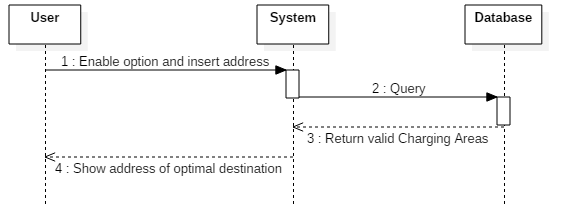
\includegraphics[width=\linewidth,keepaspectratio]{../Diagrams/SD/UC_13.png}
\caption{Use Case 13}
\end{figure}
\FloatBarrier

\clearpage
\subsubsection{Class Diagram}
\begin{figure}[h]
\centering
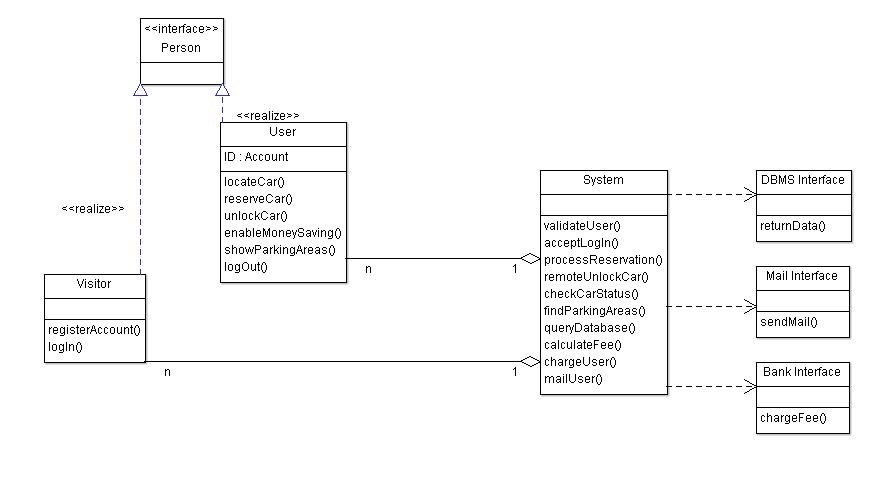
\includegraphics[width=\linewidth,keepaspectratio]{../Diagrams/CD/Class_Diagram.png}
\caption{Class Diagram}
\end{figure}
\FloatBarrier

\clearpage
\subsubsection{Statechart Diagram}
\begin{figure}[h]
\centering
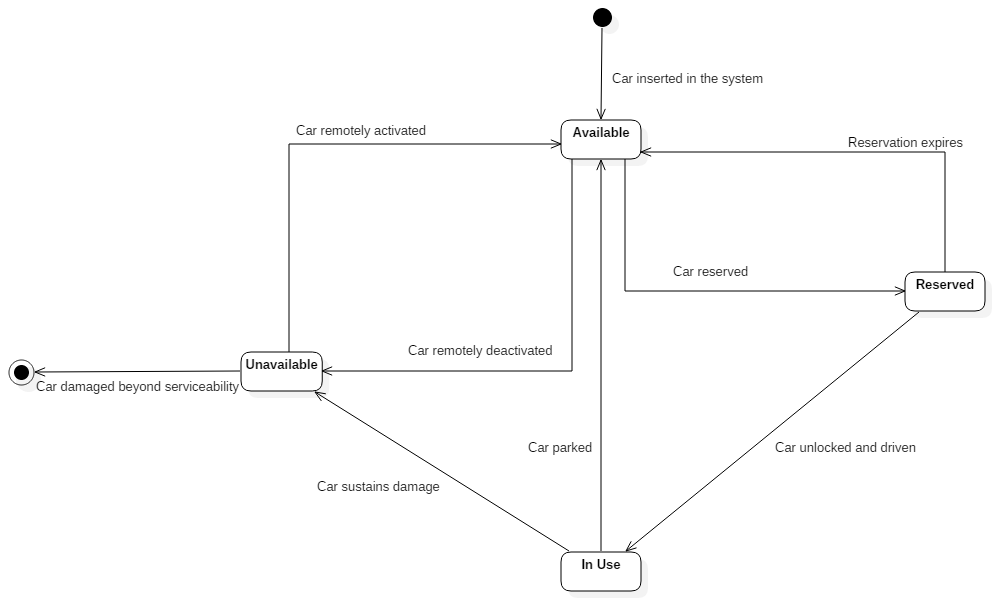
\includegraphics[width=\linewidth,keepaspectratio]{../Diagrams/SCD/SCD_Car.png}
\caption{Statechart diagram of Car}
\end{figure}
\FloatBarrier

\subsubsection{Traceability Matrix}
%TODO Traceability Matrix
\newcounter{idcounter}
\begin{center}
  \begin{longtable}{|p{.15\textwidth}|p{.12\textwidth}|p{.26\textwidth}|p{.23\textwidth}|p{.26\textwidth}|}
    \hline
    \stepcounter{idcounter}
    \textbf{Raw ID} & \textbf{Goal ID} & \textbf{Requirement ID} & \textbf{Use Case ID}   \\ \hline   
    \theidcounter & G1 & R1 & UC1 \\ \hline
    \stepcounter{idcounter}
    \theidcounter & G1 & R1 & UC2 \\ \hline
    \stepcounter{idcounter}
    \theidcounter & G2 & R1 & UC3 \\ \hline
    \stepcounter{idcounter}
    \theidcounter& G3 &  R2 & UC6\\ \hline
    \stepcounter{idcounter}
    \theidcounter & G4 & & UC7\\ \hline
    \stepcounter{idcounter}
    \theidcounter & G5 & & UC8\\ \hline
    \stepcounter{idcounter}
    \theidcounter & G6 & & UC8\\ \hline
    \stepcounter{idcounter}
    \theidcounter & G7 & & UC9\\ \hline
    \stepcounter{idcounter}
    \theidcounter & G8 & & UC9\\ \hline
    \stepcounter{idcounter}
    \theidcounter & G9 & & UC5\\ \hline   
    \stepcounter{idcounter}
    \theidcounter & G10 & & UC11\\ \hline
    \stepcounter{idcounter}
    \theidcounter & G11 & & U10\\ \hline
    \stepcounter{idcounter}
    \theidcounter & G11 & & UC11\\ \hline
    \stepcounter{idcounter}
    \theidcounter & G12 & & UC11\\ \hline    
    \stepcounter{idcounter}
    \theidcounter & G13 & & UC11\\ \hline   
     \stepcounter{idcounter}
    \theidcounter & G13 & & UC12\\ \hline    
    \stepcounter{idcounter}
    \theidcounter & G14 & & UC11\\ \hline    
    \stepcounter{idcounter}
    \theidcounter & G15 & & UC13\\ \hline
  \end{longtable}
\end{center}

